% Foliensatz: "AFu-Kurs nach DJ4UF" von DK0TU, Amateurfunkgruppe der TU Berlin
% Lizenz: CC BY-NC-SA 3.0 de (http://creativecommons.org/licenses/by-nc-sa/3.0/de/)
% Autoren: Sebastian Lange <dl7bst@dk0tu.de>, Lars Weiler <dc4lw@darc.de>

% FIXME Durch den Merge mit Lars' Input müssen die Quellen nochmal sortiert werden!
% TODO Aufgaben in den Folien mit Skript abgleichen

\documentclass[aspectratio=169]{beamer}

\usepackage[ngerman]{babel} % deutsche Worttrennung etc.
\usepackage[utf8]{inputenc} % UTF8 Text

\usepackage[super, comma, numbers, square, sort]{natbib}

\usepackage{hyperref}       % Hyperref Package für bessere Referenzen (todo)
\hypersetup{
	colorlinks=false,       %   false: boxed links; true: colored links
    %linkcolor=white,       %   color of internal links (change box color with linkbordercolor)
    citecolor=red,          %   color of links to bibliography
    filecolor=white,        %   color of file links
    urlcolor=blue           %   color of external links
}

\usepackage{multirow}
\usepackage{wasysym}  % Math Symbols like \permil
%\usepackage{colortbl}
%\usepackage{subscript}
%\usepackage{caption}
%\usepackage{setspace}
%\usepackage{xcolor}        % benutze CodeListe

% Footnote
%\usepackage{hanging}
%
%\setbeamertemplate{footnote}{%
%  \hangpara{2em}{1}%
%  \makebox[2em][l]{\insertfootnotemark}\footnotesize\insertfootnotetext\par%
%}


%\usepackage{pgf}
%\usepackage{tikz}
%\usetikzlibrary{arrows,automata}
%\usetikzlibrary{positioning}
%
%\tikzset{
%    state/.style={
%           rectangle,
%           rounded corners,
%           draw=black, very thick,
%           minimum height=2em,
%           minimum width=2pt,
%           inner sep=2pt,
%           text centered,
%           },
%}

%\usepackage{listings}
%\lstset{basicstyle=\small, numberstyle=\tiny, extendedchars=true, numbers=left, numbersep=5pt}
%\lstset{showtabs=false, showspaces=false, showstringspaces=false}
%%\lstset{backgroundcolor=\color{white!75!lightgray}, , frame=single}
%%\lstset{backgroundcolor=\color{white}}
%%\lstset{backgroundcolor=none}
%\lstset{keywordstyle=\color{blue!50!gray},  identifierstyle=\color{black}}
%\lstset{commentstyle=\color{green!50!gray}, stringstyle=\color{red!50!gray}}
%\lstset{language=C, fontadjust=true, tabsize=2, breaklines=true}
%\lstset{backgroundcolor=\color{white!75!lightgray}, caption=\lstname, frame=single}
%\lstset{emphstyle=\color{black}\fbox}
%
%% Keine "Listing:"-Caption
%\captionsetup{labelformat=empty,labelsep=none}
%
%% für mathematische Umgebungen
%\usepackage{amsmath,amsfonts,amssymb}
%
%\lstdefinestyle{Bash}{
%language=Bash,
%frame=single,
%rulecolor=\color{black},
%backgroundcolor=\color{gray!50},
%keywordstyle=\color{black},
%identifierstyle=,
%commentstyle=\color{black},
%stringstyle=\color{magenta!65!white},
%showstringspaces=false,
%basicstyle=\footnotesize\ttfamily\color{black},
%numbers=none,
%breaklines=true,
%captionpos=b
%}

%\usepackage{listings}
%
%\lstdefinestyle{basic}{
%    captionpos=t,%
%    basicstyle=\footnotesize\ttfamily,%
%    numberstyle=\tiny,%
%    numbers=left,%
%    stepnumber=1,%
%    frame=single,%
%    showspaces=false,%
%    showstringspaces=false,%
%    showtabs=false,%
%    %
%    keywordstyle=\color{blue},%
%    identifierstyle=,%
%    commentstyle=\color{gray},%
%    stringstyle=\color{magenta}%
%}



% fließende Boxen haben keinen Abstand
%\fboxsep0mm

% inkludiere Creative Commons Helper
%%%%%%%%%%%%%%%%%%%%%%%%%%%%%%%%%%%%%%%%%%%%%%%%%%%%%%%%%%%%%%%%
%% ccBeamer 0.1, 2007-07-02                                   %%
%% Written by Sebastian Pipping <webmaster@hartwork.org>      %%
%% ---------------------------------------------------------- %%
%% Licensed under Creative Commons Attribution-ShareAlike 3.0 %%
%% http://creativecommons.org/licenses/by-sa/3.0/             %%
%%%%%%%%%%%%%%%%%%%%%%%%%%%%%%%%%%%%%%%%%%%%%%%%%%%%%%%%%%%%%%%%


%% Images
\newcommand{\CcImageBy}[1]{%
	
\includegraphics[scale=#1]{texdata/creative_commons/cc_by_30.pdf}%
}
\newcommand{\CcImageCc}[1]{%
	
\includegraphics[scale=#1]{texdata/creative_commons/cc_cc_30.pdf}%
}
\newcommand{\CcImageDevNations}[1]{%
	
\includegraphics[scale=#1]{texdata/creative_commons/cc_dev_nations_30.pdf}%
}
\newcommand{\CcImageNc}[1]{%
	
\includegraphics[scale=#1]{texdata/creative_commons/cc_nc_30.pdf}%
}
\newcommand{\CcImageNd}[1]{%
	
\includegraphics[scale=#1]{texdata/creative_commons/cc_nd_30.pdf}%
}
\newcommand{\CcImagePd}[1]{%
	
\includegraphics[scale=#1]{texdata/creative_commons/cc_pd_30.pdf}%
}
\newcommand{\CcImageSa}[1]{%
	
\includegraphics[scale=#1]{texdata/creative_commons/cc_sa_30.pdf}%
}
\newcommand{\CcImageSampling}[1]{%
	
\includegraphics[scale=#1]{texdata/creative_commons/cc_sampling_30.pdf}%
}
\newcommand{\CcImageSamplingPlus}[1]{%
	
\includegraphics[scale=#1]{texdata/creative_commons/cc_sampling_plus_30.pdf}%
}


%% Groups
\newcommand{\CcGroupBy}[2]{% zoom, gap
	\CcImageCc{#1}\hspace*{#2}\CcImageBy{#1}%
}
\newcommand{\CcGroupByNc}[2]{% zoom, gap
	\CcImageCc{#1}\hspace*{#2}\CcImageBy{#1}\hspace*{#2}\CcImageNc{#1}%
}
\newcommand{\CcGroupByNcNd}[2]{% zoom, gap
	\CcImageCc{#1}\hspace*{#2}\CcImageBy{#1}\hspace*{#2}\CcImageNc{#1}\hspace*{#2}\CcImageNd{#1}%
}
\newcommand{\CcGroupByNcSa}[2]{% zoom, gap
	\CcImageCc{#1}\hspace*{#2}\CcImageBy{#1}\hspace*{#2}\CcImageNc{#1}\hspace*{#2}\CcImageSa{#1}%
}
\newcommand{\CcGroupByNd}[2]{% zoom, gap
	\CcImageCc{#1}\hspace*{#2}\CcImageBy{#1}\hspace*{#2}\CcImageNd{#1}%
}
\newcommand{\CcGroupBySa}[2]{% zoom, gap
	\CcImageCc{#1}\hspace*{#2}\CcImageBy{#1}\hspace*{#2}\CcImageSa{#1}%
}
\newcommand{\CcGroupDevNations}[2]{% zoom, gap
	\CcImageCc{#1}\hspace*{#2}\CcImageDevNations{#1}%
}
\newcommand{\CcGroupNcSampling}[2]{% zoom, gap
	\CcImageCc{#1}\hspace*{#2}\CcImageNc{#1}\hspace*{#2}\CcImageSampling{#1}%
}
\newcommand{\CcGroupPd}[1]{% zoom
	\CcImagePd{#1}%
}
\newcommand{\CcGroupSampling}[1]{% zoom
	\CcImageSampling{#1}%
}
\newcommand{\CcGroupSamplingPlus}[1]{% zoom
	\CcImageSamplingPlus{#1}%
}


%% Text
\newcommand{\CcLongnameBy}{Attribution}
\newcommand{\CcLongnameByNc}{Attribution-NonCommercial}
\newcommand{\CcLongnameByNcNd}{Attribution-NoDerivs}
\newcommand{\CcLongnameByNcSa}{Attribution-NonCommercial-ShareAlike}
\newcommand{\CcLongnameByNd}{Attribution-NoDerivs}
\newcommand{\CcLongnameBySa}{Attribution-ShareAlike}

\newcommand{\CcNote}[1]{% longname
	This work is licensed under the \textit{Creative Commons #1 3.0 License}.%
}


% generelles Thema auswählen
\usetheme{Goettingen} %Berlin spart ohne Sidebar allerdings angenehm Platz
% AnnArbor | Antibes | Bergen | Berkeley | Berlin | Boadilla | boxes | CambridgeUS | Copenhagen | Darmstadt | default | Dresden | Frankfurt | Goettingen | Hannover | Ilmenau | JuanLesPins | Luebeck | Madrid | Malmoe | Marburg | Montpellier | PaloAlto | Pittsburgh | Rochester | Singapore | Szeged | Warsaw

% Farben wählen
\usecolortheme{beetle}
% beaver | beetle | crane | default | dolphin | dove | fly | lily | orchid | rose | seagull | seahorse | sidebartab | structure | whale | wolverine

% Setze alle Farben auf Grau und Weiß
%\definecolor{craneorange}{RGB}{64,64,64}
%\definecolor{craneblue}{RGB}{255,255,255}

% Schriftart wählen
\usefonttheme{default}
% default | professionalfonts | serif | structurebold | structureitalicserif | structuresmallcapsserif

% Innere Themen(Kopf-, Fuß-, Sidebar usw)
%\useinnertheme{default}
\useinnertheme{circles}
% default | inmargin | rectangles | rounded | circles

% Äußere Themen (Anordnung der inneren, grenzen der Folien etc.)
\useoutertheme{infolines}
% default | infolines | miniframes | shadow | sidebar | smoothbars | smoothtree | split | tree

% Deaktiviere Navigations-Symbole ({} -> leer)
\setbeamertemplate{navigation symbols}{}
%\setbeamertemplate{navigation symbols}{\large \ifnum \insertframenumber <10 0\fi\insertframenumber/\inserttotalframenumber\vspace*{0.2ex}}

% Zeige ein Hintergrundbild
\setbeamertemplate{background canvas}{
        \hspace*{-2.0cm}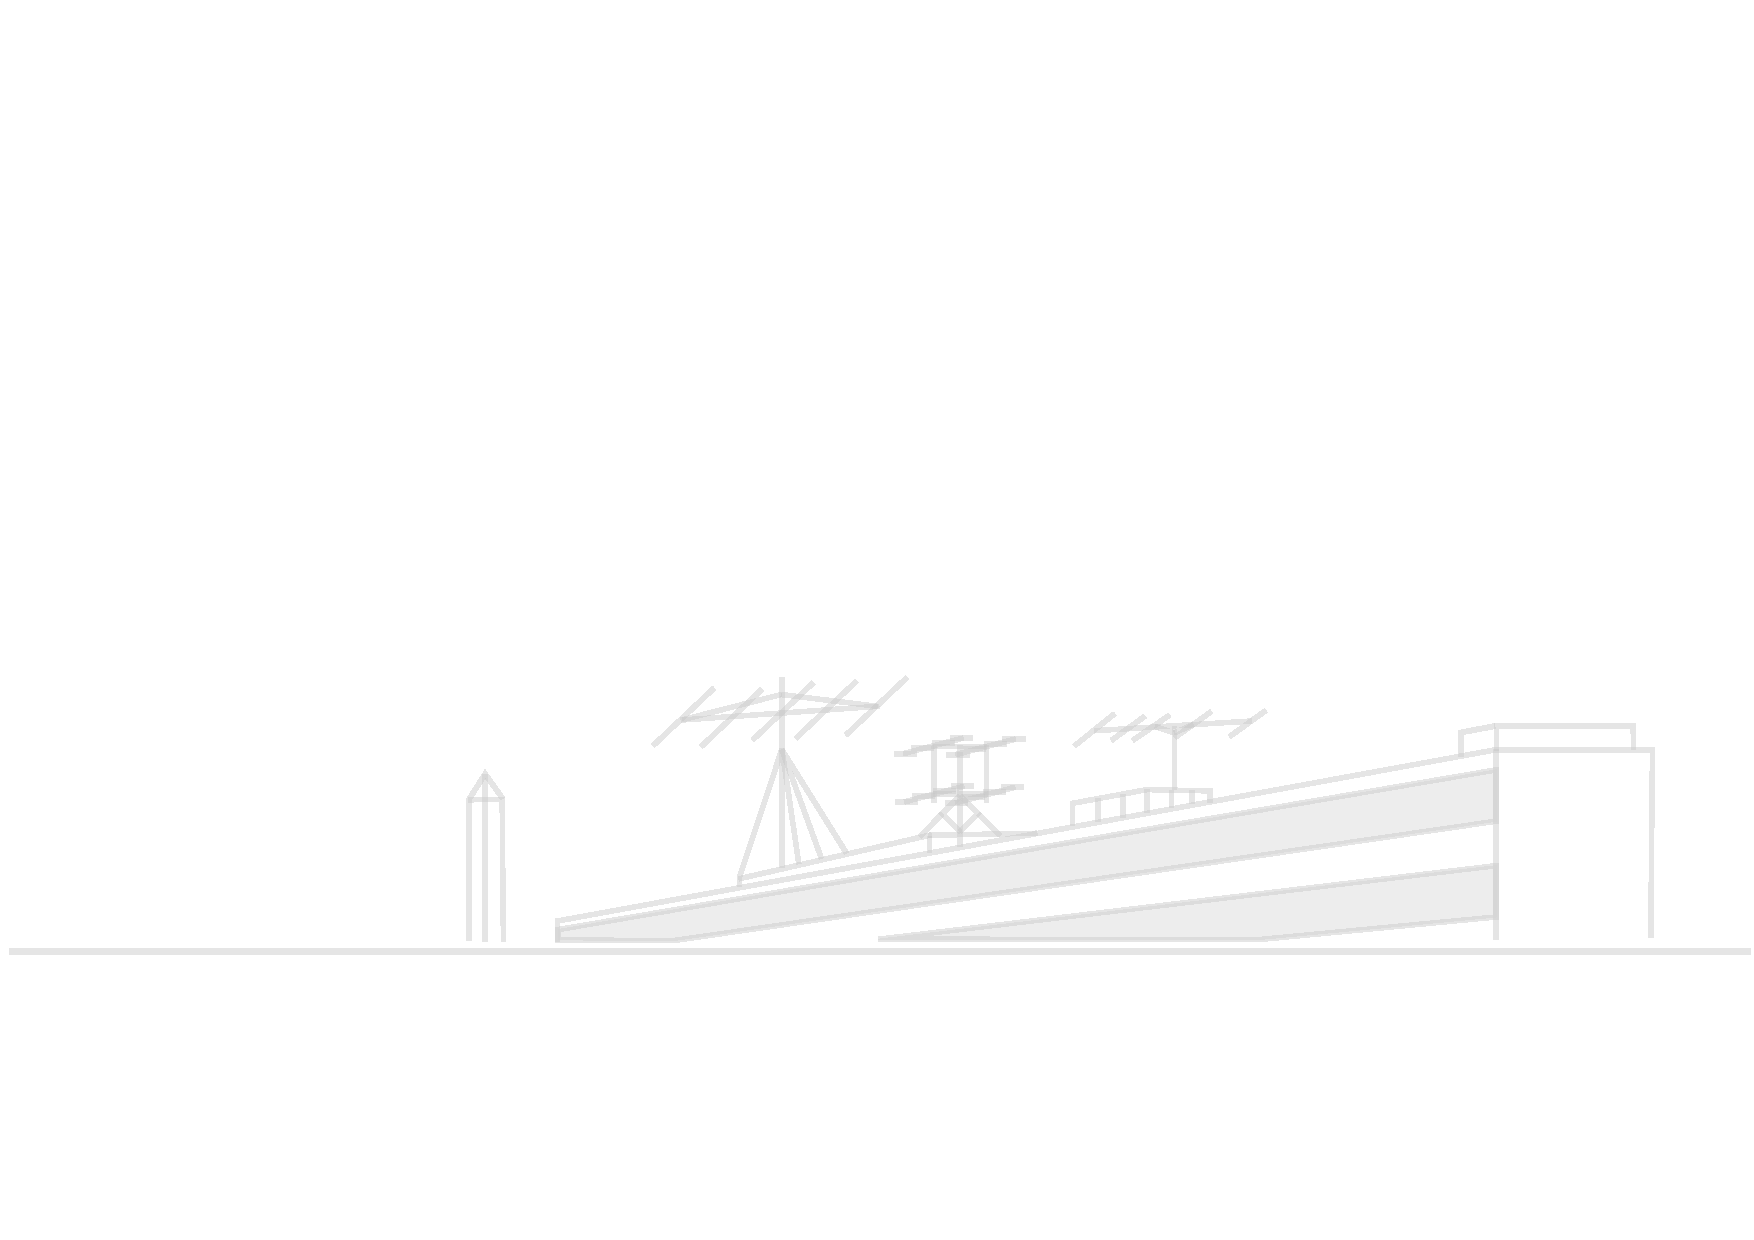
\includegraphics[width=17.8cm]{texdata/dk0tu_rooftop_background.pdf}
}

% Foliennummer einfügen
\setbeamertemplate{footline}[frame number]
%\setbeamertemplate{footline}{}

% Ändere das Zeichen vor jedem item
%\setbeamertemplate{itemize item}{\color{craneorange}$\blacktriangleright$}
%\setbeamertemplate{itemize subitem}{\color{craneorange}$\triangleright$}
%\setbeamertemplate{itemize subsubitem}{\color{craneorange}$\blacktriangleright$}

% Ändert die Blöcke 
\setbeamertemplate{blocks}[rounded][shadow=true]
% default | rounded [shadow=true|false]

%
% Eigene Kommandos
%

% Hack to get natbib and beamer working together. "The beamer user guide suggests
% that only the manual bibliography entry approach is supported"
% on some system it works out of the box, sometimes you need the hack :-(
% so check it --dl7bst
\ifdefined\newblock
    \relax
\else
    \newcommand{\newblock}{}
\fi

% \includedia command to generate png out of a dia file
% NEEDS installed dia and pdflatex option --shell-escape
\newcommand{\includedia}[1]{
    \immediate\write18{/usr/bin/dia #1.dia -e #1_diatmp.png -t png}
}

% RICHIG GROSSER FONT!
\newfont{\bigfont}{cmr10 at 144pt}
\newfont{\smallfont}{cmr10 at 8pt}

% Römische Ziffern
\makeatletter
\newcommand{\rmnum}[1]{\romannumeral #1}
\newcommand{\Rmnum}[1]{\expandafter\@slowromancap\romannumeral #1@}
\makeatother

% Schwarze Überschrift
%\setbeamercolor{frametitle}{fg=black}
%\setbeamercolor{title}{fg=black}

% Item- und Box-Farben
\definecolor{deepBlue}{HTML}{000066}
\setbeamercolor{itemize item}{fg=deepBlue}
\setbeamercolor{itemize subitem}{fg=deepBlue}
\setbeamercolor{description item}{fg=deepBlue}
\setbeamercolor{block title}{fg=deepBlue!100, bg=blue!15}
\setbeamercolor{block body}{fg=black, bg=blue!5}
\setbeamercolor{block title alerted}{fg=deepBlue, bg=red!75}
\setbeamercolor{block body alerted}{fg=black, bg=red!15}
\setbeamercolor*{block title example}{fg=blue!50, bg=blue!10}
\setbeamercolor*{block body example}{fg= blue, bg=blue!5}

%\setbeamercolor{section in head/foot}{parent=palette primary}
%\setbeamercolor{subsection in head/foot}{parent=palette secondary}
%\setbeamercolor{sidebar}{fg=darkblue,bg=yellow!90!orange}
%\setbeamercolor{title in sidebar}{fg=darkblue}
%\setbeamercolor{author in sidebar}{fg=darkblue}
%\setbeamercolor{section in sidebar}{fg=darkblue!10!black}
%\setbeamercolor{subsection in sidebar}{fg=darkblue!50!black}

% Titlepage Infos
\title{AFu-Kurs nach DJ4UF}
\author[DKØTU]{DKØTU\\ \footnotesize{Amateurfunkgruppe der TU Berlin}}
\institute[DKØTU]{\url{http://www.dk0tu.de} }

% PDF-Eigenschaften
\subject{DK0TU-Amateurfunkkurs nach DJ4UF}
\keywords{Amateurfunk Kurs HAM Radio Course CC-BY-NC-SA OpenSource TU Berlin DK0TU}

\subtitle{Technik Klasse A 11: \\
  Signale \\[2em]}
\date{Stand 15.06.2016}
 \begin{document}

\begin{frame}
    \titlepage
    \vfill
    \begin{center}
        \ccbyncsaeu\\
        {\tiny This work is licensed under the \em{Creative Commons Attribution-NonCommercial-ShareAlike 3.0 License}.}\\[0.5ex]
         \tiny Amateurfunkgruppe der Technische Universität Berlin (AfuTUB), DKØTU
         %\includegraphics[scale=0.5]{img/DK0TU_Logo.pdf}
    \end{center}
\end{frame}


\section{Einleitung}

\begin{frame}
  \frametitle{Einleitung}

  \centering \Large Generell: Was sind Signale?

\end{frame}

\begin{frame}
  \frametitle{Signale}

  Allgemein: Signale sind Zeichen. Ist ihre Bedeutung festgelegt können
  Nachrichten transportiert werden. \\[2em]

  Dazu ein wenig Theorie für den Bereich der elektrischen Nachrichtenübertragung...

\end{frame}

\begin{frame}
  \frametitle{Signale}

  Nachrichtentechnik: Grundsätzliche Unterscheidung zwischen
  \textbf{periodischen} und \textbf{nicht-periodischen} Signalen. \\[2em]

  Welche periodischen Signale kennt ihr?

\end{frame}

\section{Periodische Signale}


\begin{frame}
  \frametitle{Periodische Signale}

  \begin{center}
    \begin{figure}
      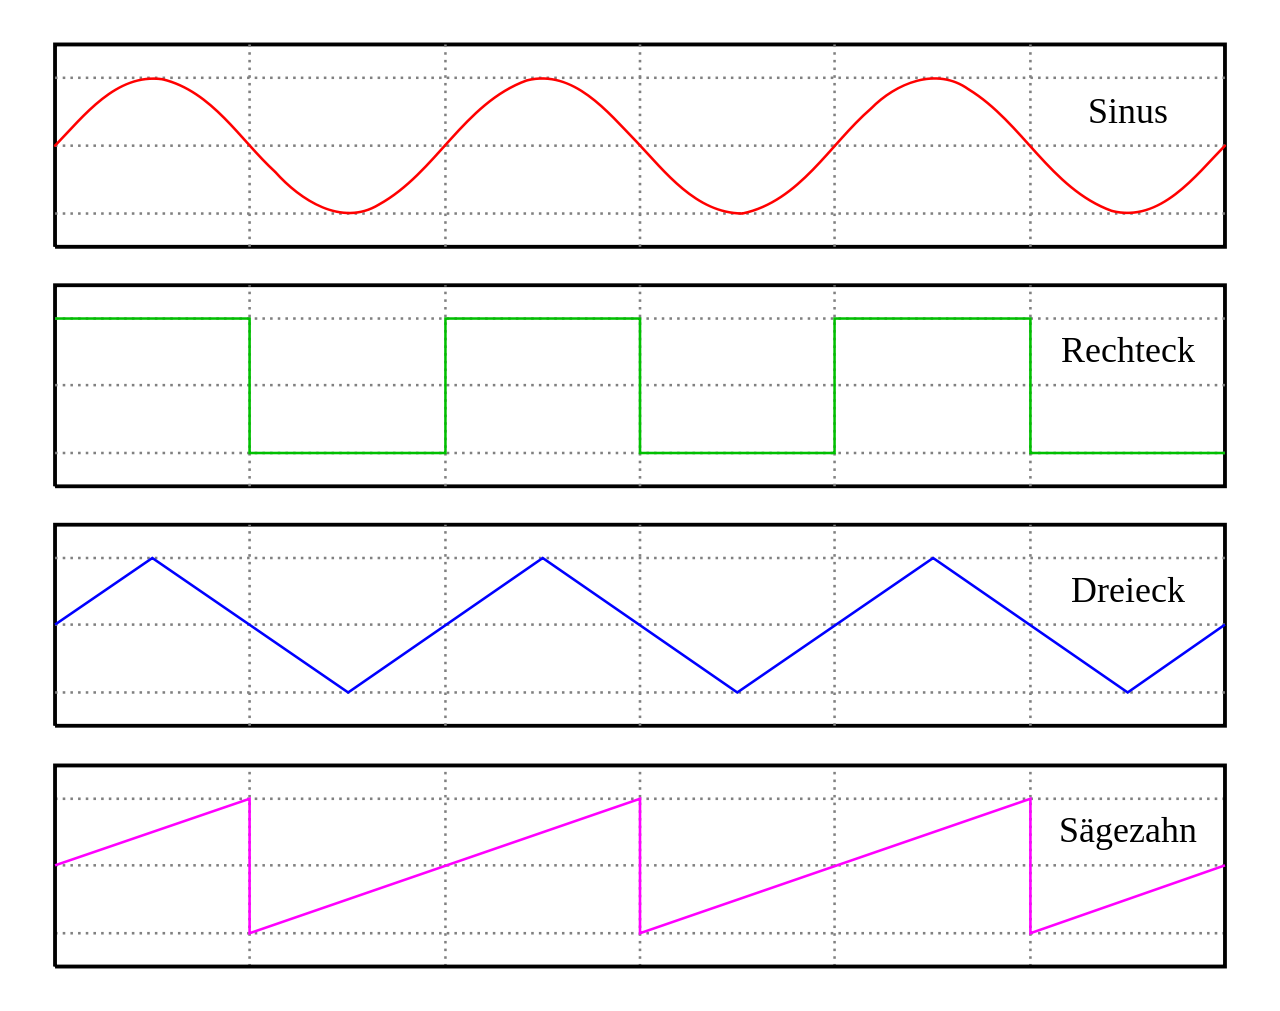
\includegraphics[width=\textwidth,height=0.7\textheight,keepaspectratio]{a11/Waveforms_de.png}
      \attribcaption{Verschiedene periodische Wellenformen}{Mik81}{https://commons.wikimedia.org/wiki/File:Waveforms_de.svg}{\ccbysa}
    \end{figure}
  \end{center}

\end{frame}

\subsection{Sinusförmig}

\begin{frame}{Sinusförmige Signale}
  Fundamental: Schallwellen und elektromagnetische Wellen lassen sich als zusammengesetzte Sinus- und Cosinuswellen beschreiben

  \begin{center}
    \begin{figure}
      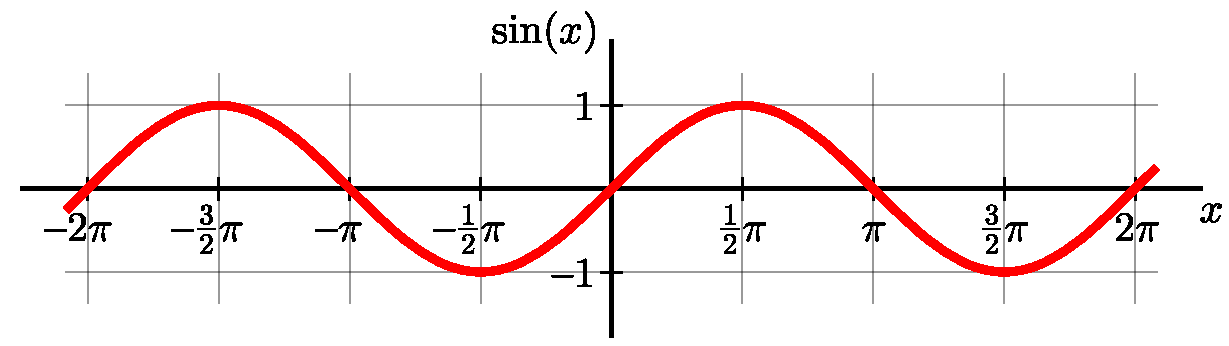
\includegraphics[width=\textwidth,height=.4\textheight,keepaspectratio]{a11/Sine.pdf}
      \attribcaption{Sinuskurve}{Geek3}{https://commons.wikimedia.org/wiki/File:Sine.svg}{\ccbysa}
    \end{figure}
  \end{center}

  Entstehung von Sinus und Cosinus am Einheitskreis, z.B. durch einen Generator (\href{https://upload.wikimedia.org/wikipedia/commons/9/9c/Einheitskreis_mit_Sinus_und_Kosinusfunktion.gif}{\ExternalLink~Animierte Grafik})

\end{frame}

\begin{frame}
  \frametitle{Sinusförmige Signale}

  \begin{center}
    \begin{figure}
      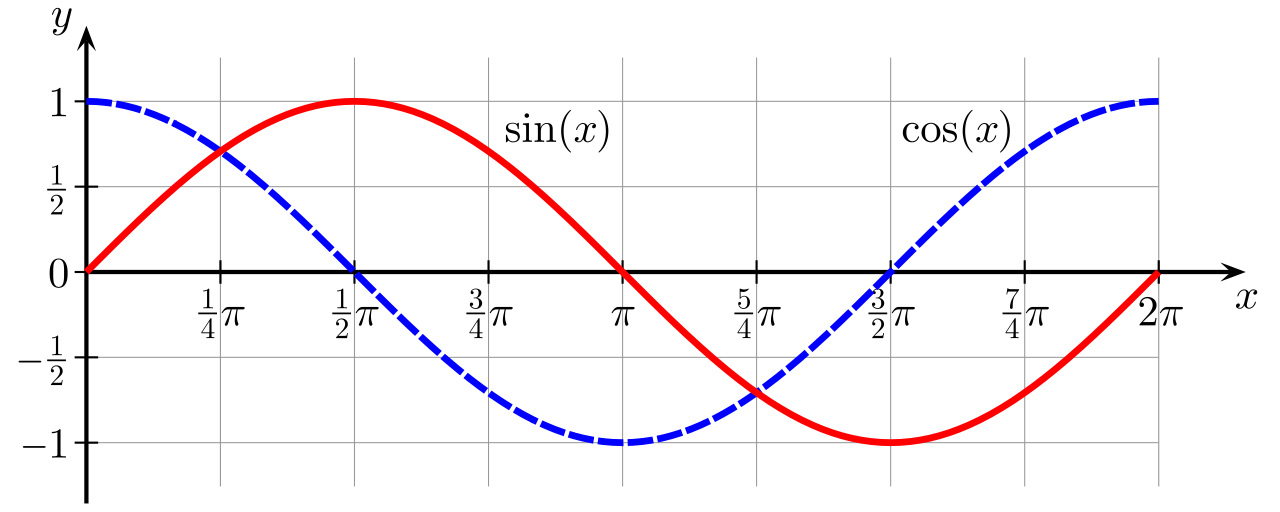
\includegraphics[width=1\textwidth,height=.55\textheight,keepaspectratio]{a11/Sine_cosine_one_period.png}
      \attribcaption{SINUS und COSINUS-Graph der Funktionen sin(x) und cos(x). Eine Periode von 0 bis 2$\pi$ ist dargestellt. Die x-Achse ist in $\pi$-Anteilen skaliert entsprechend 0 bis 2$\pi$ bzw. 0$^\circ$ bis 360$^\circ$}{Geek3}{https://commons.wikimedia.org/wiki/File:Sine_cosine_one_period.svg}{\ccby}
    \end{figure}
  \end{center}

  Was sind Amplitude, Scheitelwert, Spitze-Spitze-Wert, Periodendauer,
  Frequenz, Effektivwert?

\end{frame}

\begin{frame}{Kenngrößen}
  \begin{columns}[c]
    \column[c]{.4\textwidth}
    \begin{figure}
      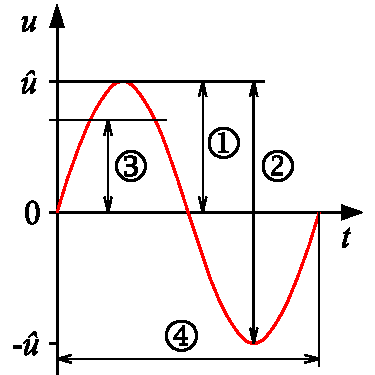
\includegraphics[width=\textwidth,height=\textheight,keepaspectratio]{a11/Sinusspannung.pdf}
      \attribcaption{Kenngrößen an sinusförmiger Wechselspannung}{Saure}{https://commons.wikimedia.org/wiki/File:Sinusspannung.svg}{\ccpd}
    \end{figure}
    \column[c]{.55\textwidth}
    \begin{block}{Begriffe}
      \begin{enumerate}
        \item Scheitelwert, Spitzenwert $\skew{4}\hat{U}$
        \item Spitze-Spitze-Wert $U_{SS} = 2 \cdot \skew{4}\hat{U}$
        \item Effektivwert $U_{eff} = \frac{\skew{4}\hat{U}}{\sqrt{2}} \approx 0,7 \cdot \skew{4}\hat{U}$
        \item Periodendauer $T = \frac{1}{f} = \frac{2\pi}{\omega}$\\
          mit Kreisfrequenz $\omega = 2\cdot\pi \cdot f$
      \end{enumerate}
    \end{block}
  \end{columns}
\end{frame}

\begin{frame}
  \begin{tabular}{l||p{.8\textwidth}}\hline
    \textbf{TB609} & \textbf{Der Spitzen-Spitzen-Wert der häuslichen 230-V-Strom"-ver"-sor"-gung ist}\\ \hline\hline
    A & 163 Volt. \\ \hline
    B & 325 Volt. \\ \hline
    C \only<2>\checkmark & 650 Volt. \\ \hline
    D & 460 Volt. \\ \hline
  \end{tabular}

  \bigskip

  \only<2>{$230V \cdot \sqrt{2} \cdot 2$ \hfill -- Darauf achten, ob vielleicht nach Spitzenwert gefragt ist.

  \vspace{3em} Generell bei Leistungsberechnungen mit Wechselströmen: Effektivwert nehmen!}
\end{frame}

% -> Aufgabenblatt
% \begin{frame}
%   \begin{tabular}{l||p{.8\textwidth}}\hline
%     \textbf{TA114} & \textbf{Die Periodendauer von $50 \mu s$ entspricht einer Frequenz von}\\ \hline\hline
%     A & 200 Hz \\ \hline
%     B & 2 kHz \\ \hline
%     C \only<2>\checkmark & 20 kHz \\ \hline
%     D & 200 MHz \\ \hline
%   \end{tabular}
% \end{frame}

\begin{frame}
  \frametitle{Sinus}

  \begin{block}{Welche Periodendauer hat europäische Netzspannung?}
    \only<1>{\vspace{1.5em}}
    \only<2>{$T = \cfrac{1}{f} = \cfrac{1}{50 Hz} \approx 20ms$}
  \end{block}

\end{frame}

\begin{frame}
  \begin{exampleblock}{Fakultative Hausaufgabe}
    Fragenkatalog Kapitel 1.2.6 Sinusförmige Signale TB601--TB612.
  \end{exampleblock}
\end{frame}

\subsubsection{Oszilloskop (Wdh.)}

\begin{frame}
  \frametitle{Kurze Wiederholung Messtechnik: Oszilloskop}

  % TODO auf entsprechenden Foliensatz referenzieren

  \begin{block}{
    Wie hoch sind Spitze-Spitze-Spannung und Frequenz?
    \begin{center}
      \begin{figure}
        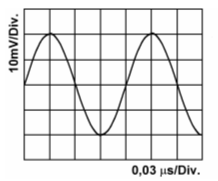
\includegraphics[width=0.5\textwidth,height=.4\textheight,keepaspectratio]{a11/TB605.png}
        \attribcaption{TB606}{BNetzA}{https://www.bundesnetzagentur.de/amateurfunk/}{}
      \end{figure}
    \end{center}
    }
    \only<1>{\vspace{2.5em}}
    \only<2>{
    $U_{SS} = 40 V$ \\
    $f = \cfrac{1}{4 \cdot 0,03 \cdot 10^{-6} s} \approx 8,33 \cdot 10^6 Hz = 8,33 MHz$
    }
  \end{block}

\end{frame}

\subsection{Phasenwinkel}

\begin{frame}
  \frametitle{Zeigerdarstellung}

  \begin{center}
    \begin{figure}
      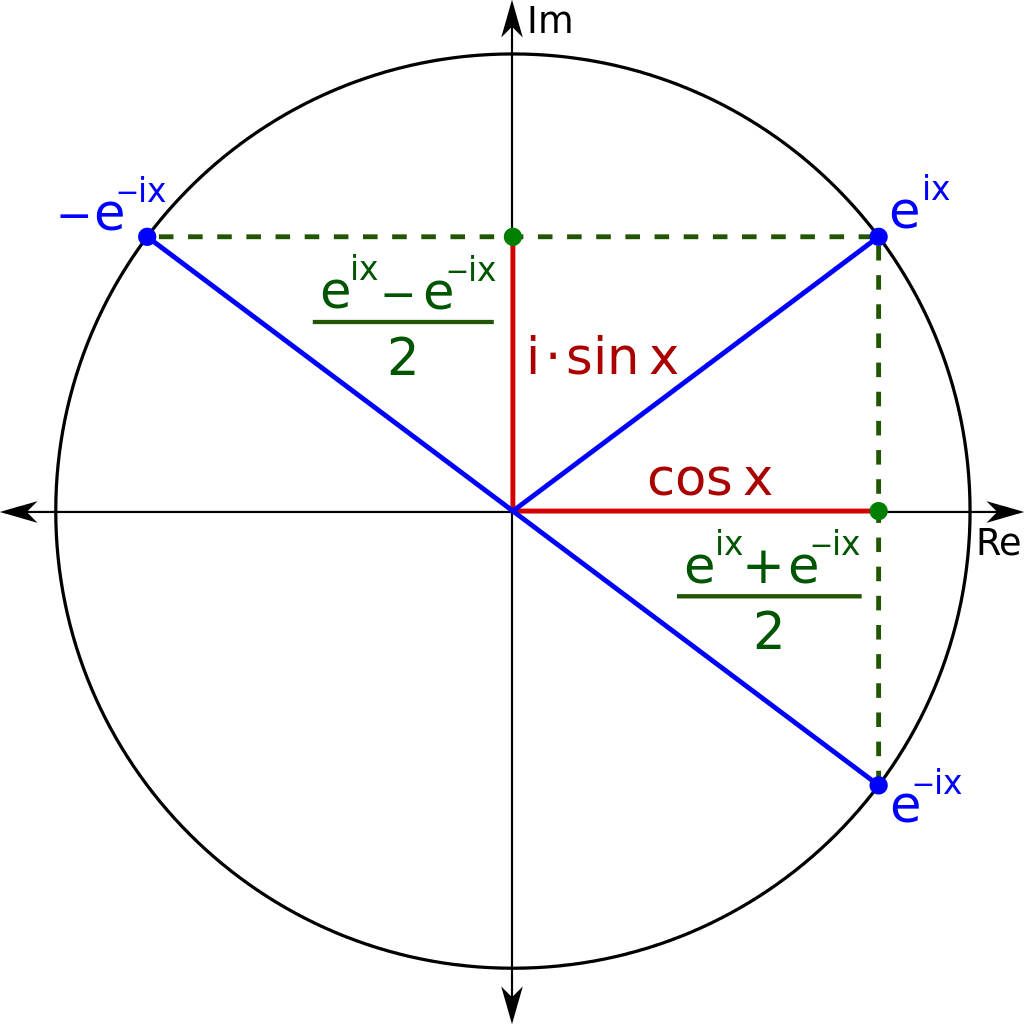
\includegraphics[width=\textwidth,height=0.5\textheight,keepaspectratio]{a11/Sine_Cosine_Exponential_qtl1.png}
      \attribcaption{Beziehung zwischen Sinus, Kosinus und Exponentialfunktion}{Quartl}{https://commons.wikimedia.org/wiki/File:Sine_Cosine_Exponential_qtl1.svg}{\ccbysa}
    \end{figure}
    \normalsize Trigonometrische Zusammenhänge im Einheitskreis.
  \end{center}

  Animationen:
  \href{http://commons.wikimedia.org/wiki/File:Einheitskreis_mit_Sinus_und_Kosinusfunktion.gif}{\ExternalLink~Wikimedia}
  und von \href{http://www.hutschdorf.de/flash/sinus.htm}{\ExternalLink~H.~Krauß (braucht Flash)}.

\end{frame}

\begin{frame}
  \frametitle{Phasenwinkel}

  \begin{block}{
    Wie groß ist folgende Phasenverschiebung?
    \begin{center}
      \begin{figure}
        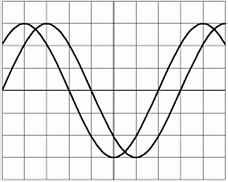
\includegraphics[width=0.5\textwidth,height=.4\textheight,keepaspectratio]{a11/TB612.png}
        \attribcaption{TB612}{BNetzA}{https://www.bundesnetzagentur.de/amateurfunk/}{}
      \end{figure}
    \end{center}
    }
    \only<1>{\vspace{1.5em}}
    \only<2>{$\Delta\varphi = \cfrac{\pi}{4} = 45 ^{\circ}$}
  \end{block}


\end{frame}

\subsection{Weitere Signale}

\begin{frame}
  \frametitle{Ableitung weiterer Signale}

  \begin{block}{Definition}
    Hat ein Signal nur eine einzige Frequenz, ist es ein sinusförmiges Signal. Alle anderen Signale bestehen aus einem Frequenzgemisch.
  \end{block}

\end{frame}

\begin{frame}
  \frametitle{Ableitung weiterer Signale}

  Bedeutet alle möglichen periodischen Signale lassen sich aus Überlagerung von
  Sinussignalen ableiten:

  \begin{itemize}
    \item \textbf{Grundfrequenz}
    \item beliebige \textbf{ganzzahlige Vielfache} der Grundfrequenz \\
      (Oberwellen bzw. Harmonische)
  \end{itemize}

  \bigskip Bereits vorgestelle Beispiele: Rechteck, Dreieck, Sägezahn
\end{frame}

\begin{frame}
  \begin{center}
    \begin{figure}
      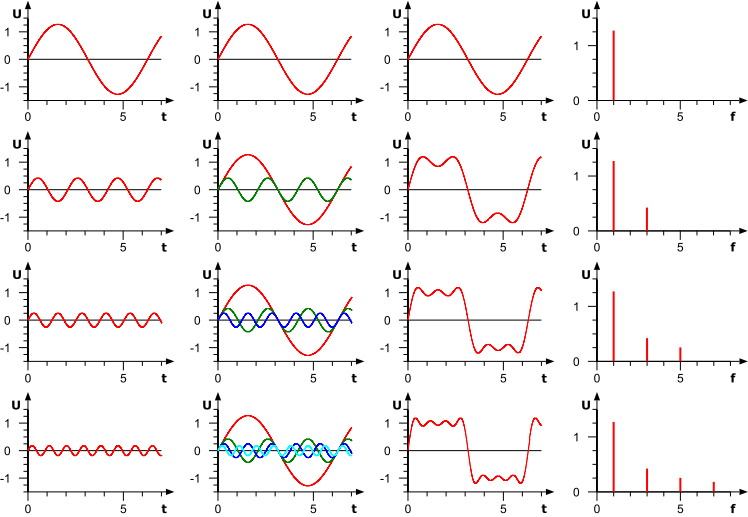
\includegraphics[width=\textwidth,height=.8\textheight,keepaspectratio]{a11/748px-Fourier_synthesis.png}
      \attribcaption{Fourieranalyse eines Rechtecksignals}{Ren\'e Schwarz}{https://commons.wikimedia.org/wiki/File:Fourier_synthesis.svg}{\ccbysa}
    \end{figure}
  \end{center}
\end{frame}

\subsubsection{Frequenzvielfache}

\begin{frame}
  \frametitle{Harmonische und Oberwellen}

  \begin{block}{Welche Frequenz hat die erste Harmonische von $430.200 MHz$?}
    \only<1>{\vspace{2em}}
    \only<2-3>{Die erste Harmonische ist die Frequenz selbst. \\
    Die erste Oberwelle bzw. zweite Harmonische liegt bei $860.4 MHz$}
  \end{block}

  \only<3>{\vspace{3em}\Large Merke: Harmonische = Oberwelle + 1}

\end{frame}

\begin{frame}{Harmonische und Oberwellen -- Beispiel: Instrumentensaite}
  \begin{columns}[c]
    \column[c]{.4\textwidth}
    \begin{figure}
      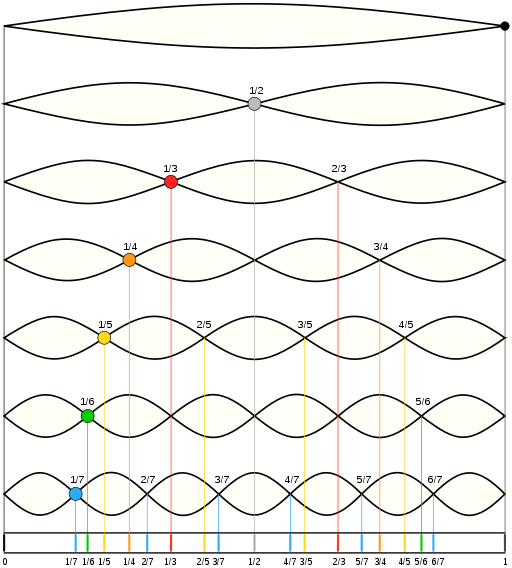
\includegraphics[width=\textwidth,height=\textheight,keepaspectratio]{a11/512px-Moodswingerscale.png}
      \attribcaption{Harmonie}{Y. Landman, verändert durch W axell}{https://commons.wikimedia.org/wiki/File:Moodswingerscale.svg}{\ccpd}
    \end{figure}
    \column[c]{.55\textwidth}
    Harmonische
    \begin{itemize}
      \item 1. Harmonische = Grundfrequenz
      \item 2. Harmonische = Doppelte Grundfrequenz
      \item 3. Harominsche = Dreifache Grundfrequenz
      \item \ldots
    \end{itemize}
    Oberwelle
    \begin{itemize}
      \item 1. Oberwelle = Doppelte Grundfrequenz
      \item 2. Oberwelle = Dreifache Grundfrequenz
      \item \ldots
    \end{itemize}
  \end{columns}
\end{frame}

% -> Skript
% \begin{frame}
%   \begin{tabular}{l||p{.8\textwidth}}\hline
%     \textbf{TB703} & \textbf{Was sind Harmonische?}\\ \hline\hline
%     A \only<2>\checkmark & Harmonische sind die ganzzahligen (1, 2, 3 \ldots) Vielfachen einer Frequenz. \\ \hline
%     B & Harmonische sind die ganzzahligen (1, 2, 3 \ldots) Teile einer Frequenz. \\ \hline
%     C & Harmonische sind die erzeugten Frequenzen oberhalb der ursprünglichen Frequenz. \\ \hline
%     D & Harmonische sind identisch mit den Oberwellen, wobei die Grundwelle keine Harmonische ist. \\ \hline
%   \end{tabular}
% \end{frame}
%
% \begin{frame}
%   \begin{tabular}{l||p{.8\textwidth}}\hline
%     \textbf{TB704} & \textbf{Die dritte Oberwelle einer Frequenz ist}\\ \hline\hline
%     A \only<2>\checkmark & die vierte Harmonische der Frequenz. \\ \hline
%     B & die dritte Harmonische der Frequenz. \\ \hline
%     C & die zweite Harmonische der Frequenz. \\ \hline
%     D & die zweite ungeradzahlige Harmonische der Frequenz. \\ \hline
%   \end{tabular}
% \end{frame}

\begin{frame}
  \begin{tabular}{l||p{.8\textwidth}}\hline
    \textbf{TA116} & \textbf{Die zweite ungeradzahlige Harmonische der Frequenz 144,690 MHz ist}\\ \hline\hline
    A & 145,000 MHz \\ \hline
    B & 289,380 MHz \\ \hline
    C \only<2>\checkmark & 434,070 MHz \\ \hline
    D & 723,450 MHz \\ \hline
  \end{tabular}
\end{frame}

\begin{frame}
  \begin{exampleblock}{Fakultative Hausaufgabe}
    Fragenkatalog Kapitel 1.2.7 Nichtsinusförmige Signale TB701--TB708.
  \end{exampleblock}
\end{frame}

\subsubsection{Sägezahn}

\begin{frame}
  \frametitle{Sägezahn}

  Grundwelle + alle Harmonische reduzierter Amplitude:

  % TODO Grafik und Formel?

  \begin{columns}
    \column{.4\textwidth}
    \begin{center}
      \begin{figure}
        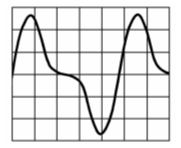
\includegraphics[width=\textwidth,height=0.6\textheight,keepaspectratio]{a11/TB705.png}
        \attribcaption{TB705}{BNetzA}{https://www.bundesnetzagentur.de/amateurfunk/}{}
      \end{figure}
    \end{center}
    \column{.6\textwidth}
    \begin{itemize}
      \item 1. Harmonische, $\cfrac{1}{1}$ Amplitude (Bsp. $2kHz$)
      \item 2. Harmonische, $\cfrac{1}{2}$ Amplitude (Bsp. \only<1>{\textbf{?}}\only<2>{$4 kHz$})
      \item 3. Harmonische, $\cfrac{1}{3}$ Amplitude
      \item ...
    \end{itemize}
  \end{columns}
\end{frame}

\subsubsection{Rechteck}

\begin{frame}
  \frametitle{Rechteck}

  Grundwelle + ungeradzahlige Harmonische:

  % TODO Grafik und Formel?

  \begin{columns}
    \column{.4\textwidth}
    \begin{center}
      \begin{figure}
        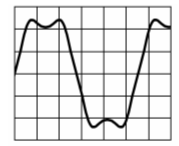
\includegraphics[width=\textwidth,height=0.6\textheight,keepaspectratio]{a11/TB706.png}
        \attribcaption{TB706}{BNetzA}{https://www.bundesnetzagentur.de/amateurfunk/}{}
      \end{figure}
    \end{center}
    \column{.6\textwidth}
    \begin{itemize}
      \item 1. Harmonische, $\cfrac{1}{1}$ Amplitude (Bsp. $2kHz$)
      \item 3. Harmonische, $\cfrac{1}{3}$ Amplitude (Bsp. \only<1>{\textbf{?}}\only<2>{$6 kHz$})
      \item 5. Harmonische, $\cfrac{1}{5}$ Amplitude
      \item ...
    \end{itemize}
  \end{columns}
\end{frame}

\section{Nicht-periodische Signale}

\begin{frame}
  \frametitle{Nicht-periodische Signale}

  \begin{block}{Definition}
    Signale, die sich nicht regelmäßig wiederholen werden nicht-periodische Signale genannt.
  \end{block}

\end{frame}

\begin{frame}
  \frametitle{Nicht-periodische Signale}

  Dies können nicht wiederkehrende Signale beliebiger Form sein, z.B. Impulse.

  \begin{center}
    \begin{figure}
      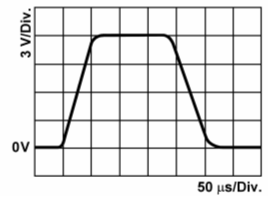
\includegraphics[width=\textwidth,height=0.5\textheight,keepaspectratio]{a11/TB702a.png}
        \attribcaption{TB702a}{BNetzA}{https://www.bundesnetzagentur.de/amateurfunk/}{}
    \end{figure}
  \end{center}

  Messung Impulsdauer oder Pulsbreite bei ca. 50\% der Amplitude.

  Wie breit ist das Signal im Beispiel? \only<2>{Antwort: $0,2 ms$}

\end{frame}

\begin{frame}
  \frametitle{Nicht-periodische Signale (nicht prüfungsrelevant)}
  \begin{columns}
    \column{.5\textwidth}
    \begin{center}
      \begin{figure}
        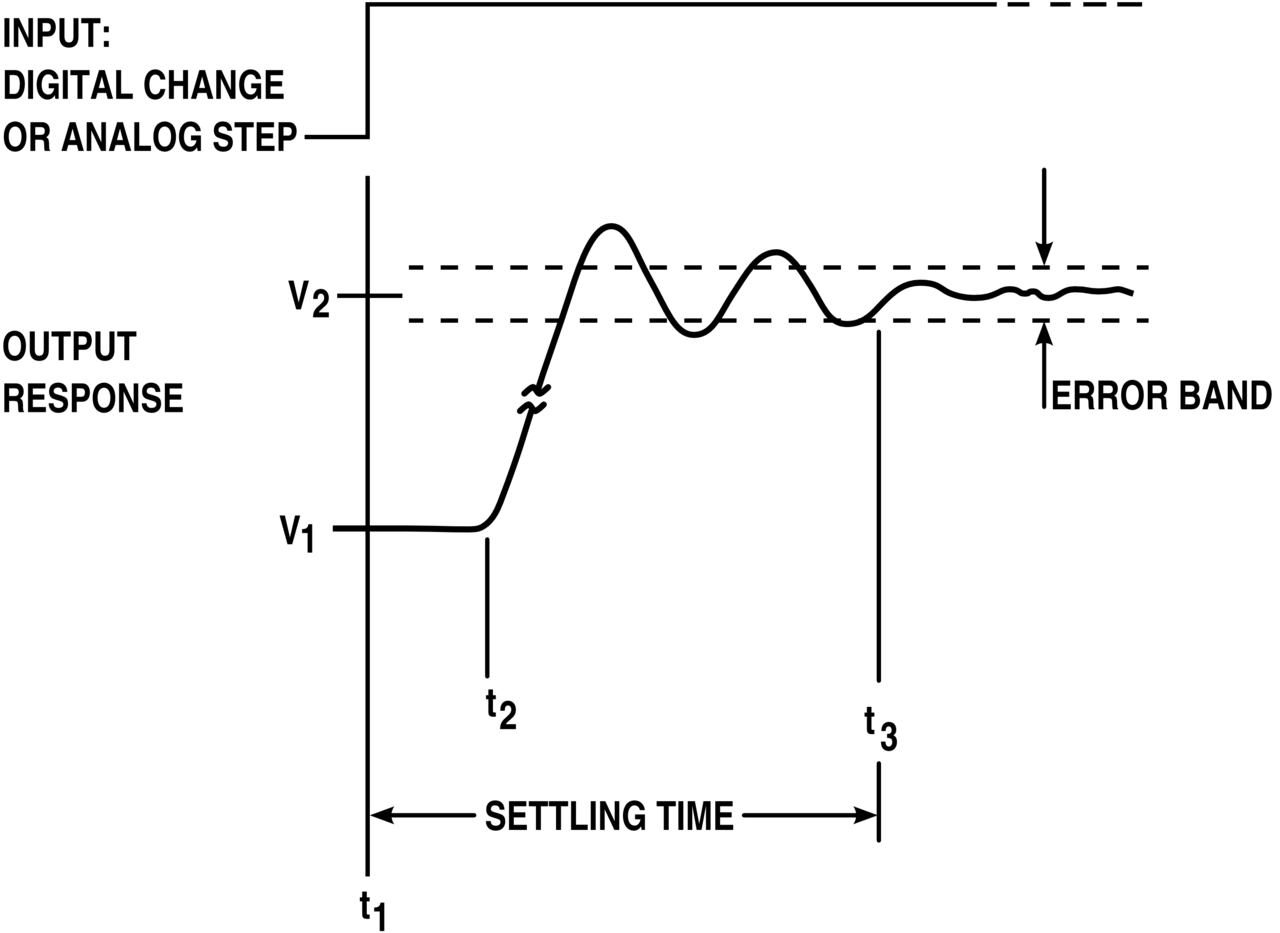
\includegraphics[width=\textwidth,height=0.7\textheight,keepaspectratio]{a11/High_accuracy_settling_time_measurements_figure_1.png}
        \attribcaption{High accuracy  settling time measurements}{Howard K. Schoenwetter}{https://commons.wikimedia.org/wiki/File:High_accuracy_settling_time_measurements_figure_1.png}{\ccpd}
      \end{figure}
    \end{center}
    \column{.5\textwidth}
    Zur Messung von Impulsantworten oder Übergangsfunktionen (Sprungantwort)
    spielen Dirac-Impuls und Heaviside-Funktion eine große Rolle. \\[2em]
    Praxis: \textbf{Sprungantwort aus Rechteck} - überführbar zu Impulsantwort.
  \end{columns}
\end{frame}

\section{Modulierte Signale}

\begin{frame}
  \frametitle{Modulation}

  \begin{block}{Bekanntes Wissen aus Technik Klasse E Lektion 14:}
    Modulation ist das "`Aufprägen"' von Signalen auf einen periodischen Träger
    durch Mischung/Multiplikation. Mischung sorgt immer für Spiegelfrequenzen.
  \end{block}

  \bigskip Im einfachen reellen Fall betrachtet (Formel nicht prüfungsrelevant):

  \begin{equation*}
    u = \skew{4}\hat{u} \cdot sin(\omega t + \varphi)
  \end{equation*}

  % TODO Parameter erläutern
  \vspace{2em}
  Welche Parameter lassen sich modulieren?

\end{frame}

\begin{frame}{Modulierte Signale}
  \begin{block}{Definition}
    Eine Kombination aus einem sinusförmigen Signal, weiteren sinusförmigen Signalen oder nicht-sinusförmigen Signalen oder Impulsen wird moduliertes Signal genannt. Es ist keine Kombination aus Harmonischen.
  \end{block}
  \vspace{2em}
  Veränderbare Kenngrößen eines Signals:
  \begin{itemize}
    \item Amplitude
    \item Frequenz
    \item Phase
  \end{itemize}
  \vspace{2em}
  Verschiebung eines Signals in einen anderen Frequenzbereich.
\end{frame}

\begin{frame}{Modulationsarten (Wdh.)}
  \begin{columns}[c]
    \column[c]{.4\textwidth}
    \begin{figure}
      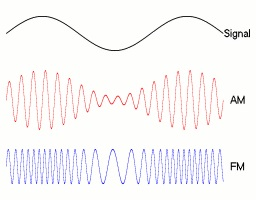
\includegraphics[width=\textwidth,height=.80\textheight,keepaspectratio]{e14/modulationen.jpg}\\
      \attribcaption{Illustration von Frequenz- und Amplitudenmodulation}{Berserkerus}{https://commons.wikimedia.org/wiki/File:Amfm3-en-de.gif}{\ccbysa}
    \end{figure}
    \column[c]{.55\textwidth}
    Amplitudenmodulation
    \begin{itemize}
      \item Zweiseitenbandmodulation
      \item Einseitenbandmodulation
      \item jeweils mit und ohne Träger
    \end{itemize}
    Winkelmodulation
    \begin{itemize}
      \item Frequenzmodulation
      \item Phasenmodulation
    \end{itemize}
  \end{columns}
\end{frame}

\subsection[AM]{Amplitudenmodulation}

\begin{frame}{Amplitudenmodulation}
  \begin{columns}[c]
    \column[c]{.4\textwidth}
    \begin{figure}
      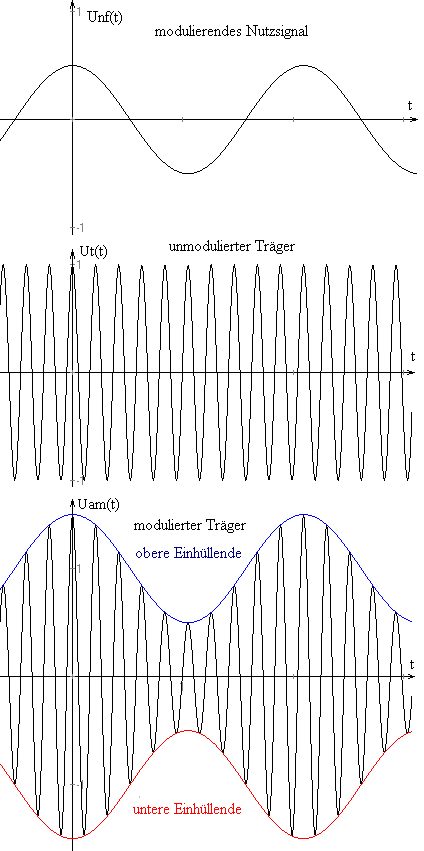
\includegraphics[width=\textwidth,height=.75\textheight,keepaspectratio]{e14/AM1.png}
      \attribcaption{Beispiel zur Amplitudenmodulation (m=0,5)}{Erico Billich}{https://commons.wikimedia.org/wiki/File:Amplitudenmodulation3.png}{\ccbysa}
    \end{figure}
    \column[c]{.55\textwidth}
    \begin{itemize}
      \item niederfrequentes Signal wird als Hüllkurve auf den Träger geprägt
        \\ $\rightarrow$ einfache Gleichrichtung zur Demodulation
      \item gleiche Information in jedem Seitenband
      \item nur maximal 18\% der Sendeleistung überträgt Information
      \item Bandbreite doppelt so groß wie maximale Modulationsfrequenz $B = 2 \cdot f_{mod max}$
      \item starke Störungsanfälligkeit
    \end{itemize}
  \end{columns}
\end{frame}

\begin{frame}
  \frametitle{Amplitudenmodulation}

  Arten:

  \begin{itemize}
    \item AM mit Träger ($> 2 \cdot$ NF-Bandbreite)
    \item AM ohne Träger aka DSB ($> 2 \cdot$ NF-Bandbreite)
    \item SSB: LSB/USB ($\approx$ NF-Bandbreite)
  \end{itemize}

  % TODO Skizzen

  \vspace{2em} Woraus ergeben sich die Bandbreiten?

\end{frame}

\subsection[SSB]{Einseitenbandmodulation}

\begin{frame}{Einseitenbandmodulation (SSB)}

  \begin{itemize}
    \item ein Seitenband unterdrücken
    \item halbiert die Bandbreite (vereinfacht)
    \item Bandbreite ist nun so groß wie das NF-Signal
  \end{itemize}

  \bigskip Für den Betrieb interessant: Lower Side Band (LSB) bei $<10MHz$, Upper Side Band (USB) bei $>10MHz$

\end{frame}

\begin{frame}{Einseitenbandmodulation (SSB)}
  \begin{center}
    \begin{figure}
      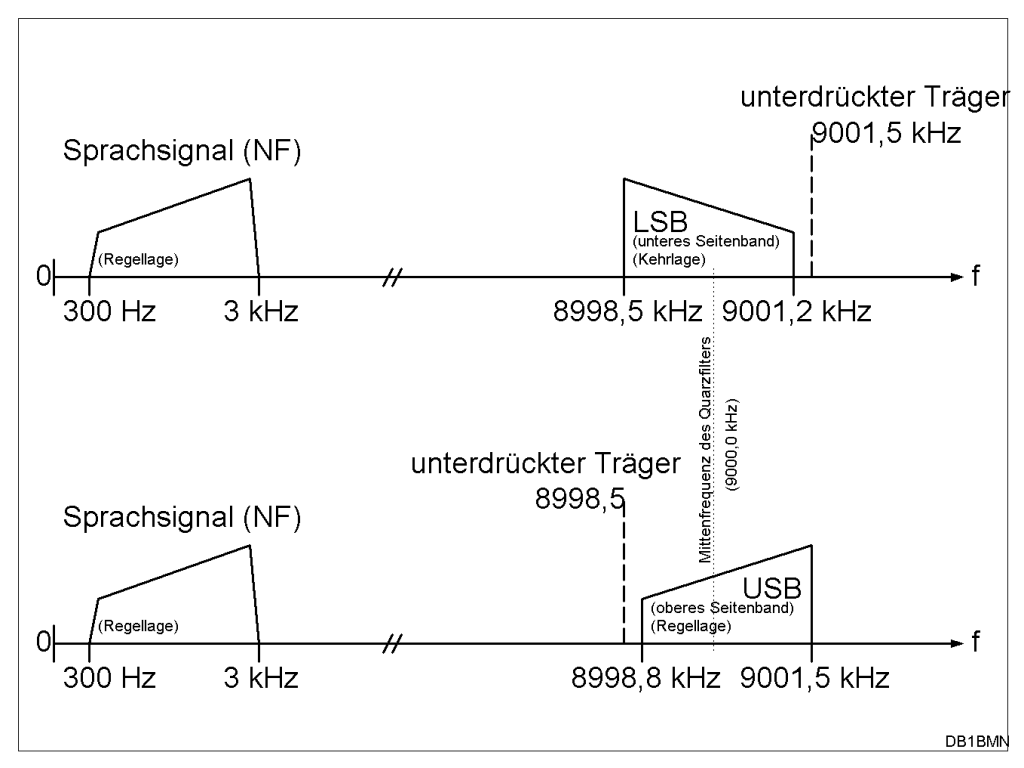
\includegraphics[width=1\textwidth,height=.75\textheight,keepaspectratio]{e16/Ssb-de.png}
      \attribcaption{Verfahren zur Erzeugung eines SSB-Signals nach der Filtermethode (stark vereinfacht).}{DB1BMN}{https://commons.wikimedia.org/wiki/File:Ssb-de.png}{\ccpd}
    \end{figure}
  \end{center}
\end{frame}

\begin{frame}
  \begin{exampleblock}{Hausaufgabe}
    Fragenkatalog Kapitel 1.5.1 Amplitudenmodulation TE101--TE113.
  \end{exampleblock}
\end{frame}

\subsection[FM]{Frequenzmodulation}

\begin{frame}{Frequenzmodulation}
  \begin{center}
    \begin{figure}
      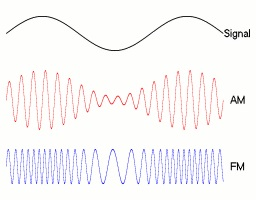
\includegraphics[width=\textwidth,height=.4\textheight,keepaspectratio]{e14/modulationen.jpg}
      \attribcaption{Illustration von Frequenz- und Amplitudenmodulation}{Berserkerus}{https://commons.wikimedia.org/wiki/File:Amfm3-en-de.gif}{\ccbysa}
    \end{figure}
    \begin{itemize}
      \item wird im VHF\,/\,UHF Bereich \& $10m$ angewandt
      \item vor allem bei mobilem Funkbetrieb
      \item findet auch bei Packet-Radio Anwendung
      \item Information steckt in der Frequenz
      \item Amplitude bleibt konstant
    \end{itemize}
  \end{center}
\end{frame}

\begin{frame}{Hub bei FM}
  \begin{center}
    \begin{figure}
      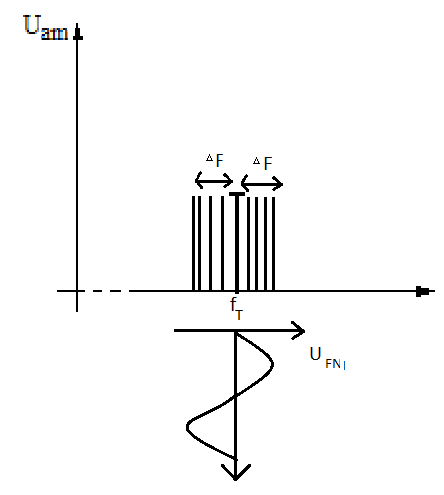
\includegraphics[width=\textwidth,height=.75\textheight,keepaspectratio]{e14/Hub.png}
      % FIXME Quelle
      \attribcaption{Hub bei FM}{Quelle unbekannt}{}{}
    \end{figure}
  \end{center}
\end{frame}

\begin{frame}{Modulationsindex}
  Verhältnis von Frequenzhub zu Modulationsfrequenz
  \begin{block}{Modulationsindex}
    $m = \cfrac{\Delta f_T}{f_{mod}}$
  \end{block}
  \begin{description}
    \item[$m\textless2$] Schmalband-FM (NFM)
    \item[$m\geq$2] Breitband-FM (WFM)
  \end{description}
  \begin{exampleblock}{Modulationsindex}
    Amateurfunk: $m = \frac{3kHz}{3kHz} = 1$\\
    UKW-Hörfunk (mono): $m = \frac{75kHz}{15kHz} = 5$\\
  \end{exampleblock}
\end{frame}

\begin{frame}{Bandbreite bei FM}
  \begin{itemize}
    \item FM erzeugt Seitenbänder
    \item Im Amateurfunk wird ein geringer Hub verwendet, der die höchste vorkommende Niederfrequenz nicht überschreitet
  \end{itemize}
  \begin{block}{Ungefähre Bandbreite (Carson Bandbreite)}
    $B = 2 \cdot (\Delta f_T + f_{mod~max})$
  \end{block}
  \begin{exampleblock}{Bandbreite}
    Amateurfunk: $B =2 \cdot (3kHz + 3kHz) = 12kHz$\\
    UKW-Hörfunk (mono): $B = 2 \cdot (75kHz + 15kHz) = 180kHz$
  \end{exampleblock}
\end{frame}

\begin{frame}{FM Vor- \& Nachteile}
  \textbf{\Large{Vorteile}}
  \begin{itemize}
    \item Störungfester, da die Amplitude konstant bleibt -- Störimpulse werden
      nicht demoduliert
  \end{itemize}
  \vspace{1cm}
  \textbf{\Large{Nachteile}}
  \begin{itemize}
    \item benötigt mehr Bandbreite
    \item nur der stärkste Sender kann empfangen werden
  \end{itemize}
\end{frame}

% -> Skript
% \begin{frame}
%   \begin{tabular}{l||p{.8\textwidth}}\hline
%     \textbf{TE206} & \textbf{FM hat gegenüber SSB den Vorteil der}\\ \hline\hline
%     A & geringeren Anforderungen an die Bandbreite. \\ \hline
%     B & größeren Entfernungsüberbrückung. \\ \hline
%     C \only<2>\checkmark & geringeren Beeinflussung durch Störquellen. \\ \hline
%     D & besseren Kreisgüte. \\ \hline
%   \end{tabular}
% \end{frame}

\begin{frame}
  \begin{tabular}{l||p{.8\textwidth}}\hline
    \textbf{TE207} & \textbf{Ein zu großer Hub eines FM-Senders führt dazu,}\\ \hline\hline
    A & dass Verzerrungen auf Grund gegenseitiger Auslöschung der Seitenbänder auftreten. \\ \hline
    B \only<2>\checkmark & dass die HF-Bandbreite zu groß wird. \\ \hline
    C & dass Verzerrungen auf Grund unerwünschter Unterdrückung der Trägerfrequenz auftreten. \\ \hline
    D & dass die Sendeendstufe übersteuert wird. \\ \hline
  \end{tabular}
\end{frame}

% Fragentyp doppelt
% \begin{frame}
%   \begin{tabular}{l||p{.8\textwidth}}\hline
%     \textbf{TE212} & \textbf{Größerer Frequenzhub führt bei einem FM-Sender zu}\\ \hline\hline
%     A & einer Reduktion der Amplituden der Seitenbänder. \\ \hline
%     B & einer Erhöhung der Amplitude der Trägerfrequenz. \\ \hline
%     C & einer Erhöhung der Senderausgangsleistung. \\ \hline
%     D \only<2>\checkmark & einer größeren HF-Bandbreite. \\ \hline
%   \end{tabular}
% \end{frame}

\begin{frame}
  \begin{tabular}{l||p{.8\textwidth}}\hline
    \textbf{TE203} & \textbf{Was gilt in etwa für die Bandbreite B eines FM-Signals, wenn der Modulationsindex $m > 2$ wird? ($f_{mod}$ sei die Modulationsfrequenz und $\Delta f$ der Hub.)}\\ \hline\hline
    A \only<2>\checkmark & $f_{mod} < \Delta f$. Die Bandbreite wird im wesentlichen durch $\Delta f$ bestimmt; $B \approx 2\cdot\Delta f$.\\ \hline
    B & $f_{mod} > \Delta f$. Die Bandbreite wird im wesentlichen durch $f_{mod}$ bestimmt; $B \approx 2\cdot f_{mod}$.\\ \hline
    C & $f_{mod} > \Delta f$. Die Bandbreite wird im wesentlichen durch $m\cdot\Delta f$ bestimmt; $B \approx m\cdot\Delta f$.\\ \hline
    D & $f_{mod} < \Delta f$. Die Bandbreite wird im wesentlichen durch $m\cdot f_{mod}$ bestimmt; $B \approx m\cdot f_{mod}$.\\ \hline
  \end{tabular}
\end{frame}

\begin{frame}
  \begin{exampleblock}{Hausaufgabe}
    Fragenkatalog Kapitel 1.5.2 Frequenzmodulation TE201--TE217.
  \end{exampleblock}
\end{frame}

\subsection[PM]{Phasenmodulation}

\begin{frame}
  \frametitle{Phasenmodulation}

  \dots ist wie die Frequenzmodulation eine Winkelmodulation und dieser sehr ähnlich. \\[4em]

  \emph{In der Prüfung spielt sie keine Rolle} -- Beispiel: PSK31

\end{frame}


\subsection{Hilfsträger}
\begin{frame}{Modulation mit Hilfsträger}
  Nutzsignal wird auf eine niederfrequente Zwischenfrequenz moduliert und danach auf AM oder FM.
  \vspace{4em}

  Beispiel: \bigskip

  1kHz Tonsignal mit Morsecode wird auf den Mikrofoneingang eines FM-Senders gelegt
  $\rightarrow$ \emph{Frequenzmodulation mit Tastung eines modulierten Hilfsträgers F2A}
\end{frame}

\begin{frame}[allowframebreaks]{Sendearten: Schlüsselzeichen}
  \emph{Wiederholung aus BV09}

  \begin{block}{Modulationsart des Hauptträgers}
    \begin{description}
      \item[A] Amplitudenmodulation
      \item[J] SSB (AM, Seitenband mit unterdrücktem Träger)
      \item[F] Winkelmodulation, Frequenzmodulation
    \end{description}
  \end{block}

  \begin{block}{Signalart}
    \begin{description}
      \item[1] Einkanaliges quantisiertes Signal ohne Hilfsträger
      \item[2] Einkanaliges quantisiertes Signal mit einem Hilfsträger
      \item[3] Einkanaliges Analogsignal
    \end{description}
  \end{block}

  \begin{block}{Informationsart}
    \begin{description}
      \item[A] Morsetelegrafie
      \item[B] Telegrafie für maschinellen Empfang (Teletype)
      \item[C] Fax
      \item[D] Daten, Telemetrie, Fernsteuerung
      \item[E] Telefonie, Rundfunk
      \item[F] Fernsehsignal
    \end{description}
  \end{block}
\end{frame}

\begin{frame}{Sendearten: Beispiele}
  \begin{exampleblock}{Beispiele für Sendearten}
    \begin{description}
      \item[A1A] CW
      \item[F2A] CW via FM-Hilfsträger
      \item[F3E] FM
      \item[J3E] SSB
      \item[J2B] RTTY
      \item[J2B] Pactor
    \end{description}
  \end{exampleblock}

  \href{https://de.wikipedia.org/wiki/Modulationsart}{\ExternalLink Übersichtliche Liste}
\end{frame}

\renewcommand{\refname}{Referenzen}

\hypertarget{refs}{}
\textcolor{white}{} \\ %\vspace{} geht nicht
\Large Referenzen/Links
\footnotesize

\begin{thebibliography}{}
  \bibitem{darc}  DARC Online-Lehrgang Klasse A:
    \url{https://www.darc.de/der-club/referate/ajw/lehrgang-ta/a11/}
  \bibitem{bna}   Fragenkatalog Bundesnetzagentur Technik Klasse A:\\
    \url{https://www.bundesnetzagentur.de/SharedDocs/Downloads/DE/Sachgebiete/Telekommunikation/Unternehmen_Institutionen/Frequenzen/Amateurfunk/Fragenkatalog/TechnikFragenkatalogKlasseAf252rId9014pdf.pdf?__blob=publicationFile&v=3}

\end{thebibliography}

% Hier könnte noch eine Kontaktfolie stehen

\end{document}

